\documentclass[a4paper,11pt,report]{article}
\usepackage[pdftex]{graphicx}
\usepackage{mathtools}
\usepackage[margin=3cm]{geometry}
\usepackage{float}
\usepackage{lscape}
\usepackage{pdfpages}
\usepackage{epsfig}
\usepackage{epstopdf}
\usepackage{amsmath}
\usepackage{sidecap}
\usepackage{hyperref}
\DeclareGraphicsExtensions{.pdf,.png,.jpg,.eps}
\setlength{\parindent}{0in}
% Alter some LaTeX defaults for better treatment of figures:
    % See p.105 of "TeX Unbound" for suggested values.
    % See pp. 199-200 of Lamport's "LaTeX" book for details.
    %   General parameters, for ALL pages:
    \renewcommand{\topfraction}{0.9}	% max fraction of floats at top
    \renewcommand{\bottomfraction}{0.8}	% max fraction of floats at bottom
    %   Parameters for TEXT pages (not float pages):
    \setcounter{topnumber}{2}
    \setcounter{bottomnumber}{2}
    \setcounter{totalnumber}{2}     % 2 may work better
    \setcounter{dbltopnumber}{2}    % for 2-column pages
    \renewcommand{\dbltopfraction}{0.9}	% fit big float above 2-col. text
    \renewcommand{\textfraction}{0.07}	% allow minimal text w. figs
    %   Parameters for FLOAT pages (not text pages):
    \renewcommand{\floatpagefraction}{0.7}	% require fuller float pages
	% N.B.: floatpagefraction MUST be less than topfraction !!
    \renewcommand{\dblfloatpagefraction}{0.7}	% require fuller float pages
\usepackage{color, colortbl}
\definecolor{Green}{rgb}{0.1,1,0.1}
\definecolor{Gray}{gray}{0.5}
\definecolor{LightGray}{gray}{0.9}

\begin{document}

\title{RentIt}
\author{Andreas P., Morten T., Mark T., Toke L. \& Mikkel F.}
\date{28-05-2013}
\maketitle

\section*{Abstract}
{
This report documents a project conducted in the fall of 2013 at the IT-University of Copenhagen. The project is a part of the course: Second Year Project: Software Development in Large Teams with International Collaboration - BNDN 2013. In the report, we (a small team of students) document our implementation of an internet radio station(RentIt), as well as our implementation of a book rental service, which we did in collaboration with students from SMU university in Singapore.\\ 
\newpage

\tableofcontents

\section{Introduction}
\subsection{Vision}
RentIt is a radio hosting service, that enables users to host online radio stations and for other users to listen to them. The creator of a channel can upload tracks to the channel, and the listeners of the channel can shape the future of the channel by submitting there up vote or down vote of a track. The service shall also promote the community by making room for discussion of channels.
It is a system intended to be used by the common user, without any special knowledge or training.

\subsection{Application scope}
In this section we will analyse what features that are needed to make a successful internet radio hosting service. We will go through the overall components that the service needs. In the requirements and use case section, we will go into more detail.

We define a internet radio hosting service as a service where users can host radio channels, define the content of the channels and where other users can listen to them. The access to the service must be accessible through a browser. The most basic component in an internet radio hosting service, is the ability to stream audio and enable users to listen to this audio in an easy and uncomplicated way. An internet radio service is different from a normal media streaming service, because several users who listen to the same radio channel must hear the exact same audio. This might seem like a small detail, but it is an aspect that requires a lot of attention. In a traditional media streaming service, the users individually stream the audio and the audio is played at individually defined intervals in the client. To emulate a traditional FM or AM radio station, we must make sure that each user listens to the exact same audio at the exact same time. 

Another crucial component is to find ways differentiate the radio stations from one another. In a radio hosting service, where users can create their own radio stations and all content on the website essentially is user created, it is important to make ways to sort the radio stations so a listener easily can find a radio station that he wants to listen to. One way to differentiate radio stations is to attach genres to the stations. This is a way for the radio hosts, to describe what kind of content a listener can expect when listening to the radio station. Another way is through subscriptions. Subscriptions serves two purposes: It gives the listener an ability to flag his favorite radio stations and enables him to access them in an easy way. It also serves as a way to rank the stations after popularity. A listener can use the subscriptions as an indication for how popular a radio stations are and use it as a guideline for finding new stations to listen to. Number of comments is also a way to find the channels that has caused the most discussions and community activity. 

This brings us to another component which is the ability for community activity between the listeners. Other user driven services, such as YouTube[reference] are very driven by their user community, and it is crucial to get a stable and active user base if your service is to be successful. To support this activity, we need to give the users the ability to make comments to channels.

We must also address the question of channel selection. How do we determine in what order the tracks on a channel should be played? On an original FM radio channel, the order of tracks is determined manually by the radio host, but on an internet radio station that is rarely an option. One solution is that the radio host makes a list of tracks and that becomes the list that is played over and over until it is changed again. This would work, but it essentially makes the radio service into an online playlist service, and that is not quite what we are going for. On a radio station the order of tracks should not be fixed and should from one hearing to another. It would be easy to do with a random generator, that simply generated a new random playlist every time the station had played through the tracks, but this would mean that popular tracks had the same chance of being played as a non popular song. Essentially, we want users to influence in what order the songs are to be played and a program that selects the songs in an intelligent and dynamic way. 

\section{Specification}
In this section we elaborate on the features discussed in the program scope section and we define the requirements and use cases. We start by defining the use cases and then we define the actual requirements based on these. 
\subsection{Use cases}
\textbf{Create account:}
The user navigates to the "create account"/"register" page. He fills out required information and agrees on possible conditions.

\textbf{Delete account:}
The user does not want to use the service any longer. He navigates to edit account and selects delete account. All data about the user is deleted accordingly.

\textbf{Listen to channel:}
The user navigates to the channel, possibly by searching for it and selects "listen to channel".

\textbf{Subscribe to channel:}
The user has selected a channel and selects "subscribe to channel". The subscription status changes accordingly.

\textbf{Unsubscribe to channel:}
The user has selected a channel he is already subscribed to and selects unsubscribe to channel. The subscription status changes accordingly.

\textbf{Comment channel:}
The user is on a channel and want to comment on it. He writes and submits the comment. The comment is saved and the page is refreshed

\textbf{Create channel:}
The user navigates to "create channel" and fills out the required information as well as uploading tracks. When the user is done it is immediately accessible by other users.

\textbf{Delete channel:}
The creater of the channel does not want the channel anymore and he decides to delete it. He navigates to edit channel and selects delete channel. All subscriptions to the channel are deleted, subscribers get notified, and the channel is removed.

\textbf{Upload track:}
The user has a channel and wants to upload a song. He navigates to edit channel. He selects the song through a filebrowser and selects upload.

\textbf{Delete track:}
The owner of a channel wants to remove a track from his channel. He navigates to edit channel. He browses the list of tracks and selects remove on the track he wants to remove.

\textbf{Edit channel:}
The owner of the channel selects edit channel and edits the channel attributes he wants to change. Then he confirmes the changes.

\textbf{Up vote/down vote track:}
The listener of a channel selects up- or down vote on a list of the last tracks that has been played.

\subsection{Functional requirements}
The functional requirements describe the required functionality of the system and defines enumerations for reference.
\\ \\
\textbf{R0:}
The system shall allow all users to create a channel, add attributes, edit and delete the channel. \\*
\textbf{Domain concepts:}
The channel shall have its own collection of tracks that it plays. It is created and maintained by the channel host(the creator of the channel).
The channel shall have genres, a description and comments posted by users.
The channel must be visible to other users with proper search parameters. \\*
\textbf{Dependencies:} 
The requirement is necessary for "upload track" and "listen to channel" because a track is associated with a channel. \\*
\textbf{Priority:} 
It is of essential importance, since the functionality is prerequested for other fundamentally important requirements.
\\ \\

\textbf{R1:}
The system shall allow users to listen to an online radio-channel that streams audio. \\*
\textbf{Domain concepts:}
A channel has a collection of tracks that can be listened to. \\*
\textbf{Priority:}
Highest as this is the primary service that the system provides. \\*
\textbf{Implementation notes:}
The system must be able to stream audio in a smooth and clutter-free manner. The system must have an intelligent way of selecting the next track to be played, meaning that it must consider up/downvotes and how much it has been played compared to other tracks of the channel.
A radio-channel must be able to stream an endless stream of audio without pauses between audio tracks.
\\ \\

\textbf{R2:}
The user shall be able to rate a track associated with a channel by up voting and down voting. \\*
\textbf{Domain concepts:}
The rating of a track must affect the frequency with which it is played within its associated channel. The user must be subscribed to the channel to vote rate an associated track.
A higher rating giving a proportionally higher chance of being played. The rating must be calculated from up votes and down votes. A user can only have one vote per track that influences the rating. \\*
\textbf{Dependencies:}
The listen to channel requirement is dependant on this requirement because the track to be played is determined by its rating.\\*
\textbf{Priority:}
It is of essential importance, since the functionality is prerequisite for other fundamentally important requirements.
\\ \\

\textbf{R3:}
It shall be possible for users with a channel to upload a track to it. \\*
\textbf{Domain concepts:}
A channel has tracks that are managed by the channel creator. \\*
\textbf{Dependencies:}
The listen to channel requirement is dependant on this requirement because the track can only be played to others if it has been uploaded to the server.\\*
\textbf{Priority:}
It is of essential importance, since the functionality is prerequisite for other fundamentally important requirements.
\\ \\

\textbf{R4:}
It shall be possible for users to subscribe and unsubscribe to channels. \\*
\textbf{Domain concepts:}
A user has a collection of subscribed channels. \\*
\textbf{Priority:}
This requirement is of secondary importance because no essential requirements are dependent on this requirement. It is important because it helps classifing popular channels and helps the user navigate to his or her favourite channels.
\\ \\

\textbf{R5:}
It shall be possible for user to comment on channels. \\*
\textbf{Domain concepts:}
A channel has comments that everyone can read and author.
\\ \\

\textbf{R6:}
It shall be possible to create, delete and edit accounts. All attributes of an account shall be editable. \\*
\textbf{Domain concepts:}
All users of the system has an account. \\*
\textbf{Dependencies:}
As an account is required for the use of the system, all requirements are dependent on the creation of an account. \\*
\textbf{Priority:} 
It is of essential importance to create an account, since the functionality is prerequisite for other fundamentally important requirements. Delete and edit are of secondary priority.
\\ \\

\textbf{R7:}
It shall be possible to search channels by a number of parameters, including number of subscribers, number of listeners, genres and name. \\*
\textbf{Priority:} 
It is of secondary importance as non of the requirements are dependent on it, and it does not provide any fundamental functionality.

\subsection{Non-functional requirements}
The non-functional requirements describes how the functionality shall work in multiple aspects, as well as defining success criteria for them. They are structured with FURPS+. \\

\textbf{Functionality} \\*
\textit{Channels} \\*
\textbf{F1:} Channel owners must be able to assign genre tags to the channels they control/own. \\*
\textbf{F2:} Users must not be required to subscribe to a channel in order to listen to it. \\*
\textbf{F3:} Users must be required to be subscribed to a channel in order to vote on the channel. \\*
\textbf{F4:} If a user unsubscribes from a channel, all votes made by that user must be removed.\\*
\textbf{F5:} Multiple users listening to the same channel at the same time must hear the same song with same amount of elapsed time (\(\Delta\) 1s), in other words, a channel is "playing" the same track for all listeners. \\*
\textbf{F6:} A list of the most popular channels should be available to all users. Popularity must be based an attribute or a combination of attributes of channels and must me documented. \\*

\textit{Tracks} \\*
\textbf{F7:} The service must support tracks in .mp3 format. \\*

\textit{Logging and Error Handling} \\*
\textbf{F8:} All exceptional states must be logged.\\*
\textbf{F9:} All state changes must be logged.\\*

\textit{Security} \\*
\textbf{F10:} All usage requires authentication. (usage meaning the use of any services related to the program)\\*

\textbf{Usability} \\*
\textbf{U1:} The website shall be intuitive to use for 90\% of persons above the age of 12 to appeal to our target audience. Intuitive means that the following use cases may take more than 3 minutes to complete.
\begin{itemize}
\item listening to a channel
\item maintaining one 
\item uploading songs
\item voting
\item subscribing
\end{itemize}

\textbf{U2:} There must be help available for all functions in the form of text. This help must be accessible from within the client \\*
\textbf{U3:} Users must be able to see all the songs contained in a channel. \\*
\textbf{U4:} Users must be able to up vote and down vote the last 5 songs that have been played on the channel while they were listening. \\*

\textbf{Reliability} \\*
\textbf{Re1:} The server must not be affected by any errors client-side. \\*
\textbf{Re2:} No system failure of any kind should affect any track in the persistence storage. \\*
\textbf{Re3:} If a channel on the server crashes:
\begin{itemize}
\item all clients must be notified about the failure.
\item the website must not be affected by the crash.
\item the website must refresh the website with possibility to listen to the channel greyed out until the channel have been fully recovered on the server side.
\item on the server side, the channel stream must shut down.
\item the error must be logged and reported automatically. 
\item the channel must be safe to use again when all track's identity have been confirmed(via hashing), and none of them are in use.
\end{itemize}
\textbf{Re4:} If upload of a track fails, everything about the track must be removed from the server and the user must be notified. \\*

\textbf{Supportability} \\*
\textbf{S1:} The server architecture must not limit the ability to correct eventual errors. This means that no unnecessary coupling exists in the server. \\*
\textbf{S2:} The server and website must be implemented modular so as to ease extendibility. This means that extensions such as video streaming or downloading of media or a non-browser-based client must not require extensive changes in the system architecture.\\*
\textbf{S3:} The impact on existing functionality of extensions and modifications shall not take more than an hour to discover for a software developer. \\*
\textbf{S4:} The server shall be running on Windows Server 2008 R2 Enterprise OS with support of .NET 4.0 Framework.\\*

\textbf{Implementaion} \\*
\textbf{I1:} Users must not be required to download or install any third party software in order to listen to a channel. \\*
\textbf{I2:} The website shall work in Google Chrome browser. \\*
\textbf{I3:} The server shall be written in C\# with the .NET 4.0 Framework and Windows Communication Foundation. \\*

\subsection{Target audience}
The target audience of our RentIt Radio system is primarily users in the age 13-35. Since our system is not just a place to listen to music, but also a place to discuss music,  older users might choose ordinary radio stations. Younger people are more used to social networks and the radio system is designed to be a social network combined with radio.

\section{Analysis}
This section contains considerations on how to implement the functional and non-functional requirements, as defined in the previous chapter. This includes the possible solutions, the chosen solution and the reasoning for the choice. We will not go into any technical specifics about the implementation, this will be covered in another chapter, but we will analyze what designs patterns, architecture and frameworks that will create the best solution. 

\subsection{Architecture}
We have several different options to consider, when choosing the right architecture for our solution. We have defined in our vision, that the solution should be an internet radio service, so it is assumed that the program most have some kind of client server architecture. A basic client/server architecture is a possible solution. The client connects to our service with a browser and the server will contain all the backend functionality as well as the generation of HTML responses. It is a simple architecture, that keeps all the functionality together, but it lacks the advantages you get from seperating the solution into smaller modules. The non-functional requirements states that the architecture must allow a non-browser-based client to connect to the server, which such a basic solution does not support. Another option is to make the core backend functionality, the functionality related to modifying, creating and deleting data, into a WCF webservice. It that case the webclient (handling all generation of HTML) makes calls to the server. A non-browser-based client could connect directly to the server without any modifications to the architecture. A disadvantage is that it makes the solution more complicated and the server responses must be designed to fit in a webservice. To even further modulate the program, you can use an external database apart from the webservice to store data. We choose to go with the most modulated solution. We let the browser call the webclient, which calls the WCF webservice, which then calls the database. More detailed description can be found in the Implementation section. \\*

\textbf{Server architecture} \\*
The largest part of our server functionality lies within the WCF webservice. It is therefore important that we analyse how this can be structured in the best way.
A WFC webservice consists of the service contracts, which defines the signatures of the webservice methods, and the actual service which contains the actual implementation of the methods. In a simple architecture you can let the webservice contain all the functionality of the service methods. This would be simple, but it would prevent the service from living up to many of the requirements we have defined in our non-functional requirements section, especially about supportability. We want the server architecture to be less coupled and more modular. The first step in modulation is to add a controller, which controls the general flow of the program. It does not contain any logic in itself, but delegates the program flow to other parts of the program, where the logic lies. It also makes sense to seperate the datastorage and the communication with the database into two different DAOs(Data Access Objects). In this way, you abstract away from the actual implementation and you make it possible to change these modules without affecting the rest of the program. Another component that it makes sense to have as a seperate module is the component responsible for handeling radio channels. Since streaming is a high-risk component of our program, it makes a lot of sense to seperate this. It open up for the possibility to modify and test the module seperately. 

\subsection{Data model}
The basic domain entities of the system consists of channel, user and track. The rest of the entities supports functionality that is required for the basic entities. \\*
User and channel each represents a unique system entity, while track can represent the exact same data as another track, only separated by the id and the channel it belongs to.
The decision to not let channels share tracks is because it would require analysis of the MP3 file to determine whether it is similar to another MP3 file, regardless of the name/artist combination.
This design does not limit a possible extension of the system to measure similar MP3 files and update references to avoid redundant data in the file system, but such an extension will not remove redundant data in the database, as our data model does not support it. 
Track has an up vote and a down vote count, which vote entities have a functional dependency to, because each vote on a track causes up vote or down vote to increase. This duplication is made in order to speed up the algorithm, because it does not need to count vote entities when it has up- and down- vote counters. \\*
The vote entity exists in order to prevent users from voting one track several times.
TrackPlay is an entity that represents a play of a track. It is an entity and not an attribute of track, because we want to record the date that the track was played. \\*
Genre is an entity and not an attribute of channel because we want to make a fixed set of genres to choose from when creating a channel.
\begin{figure}[H]
  \centering
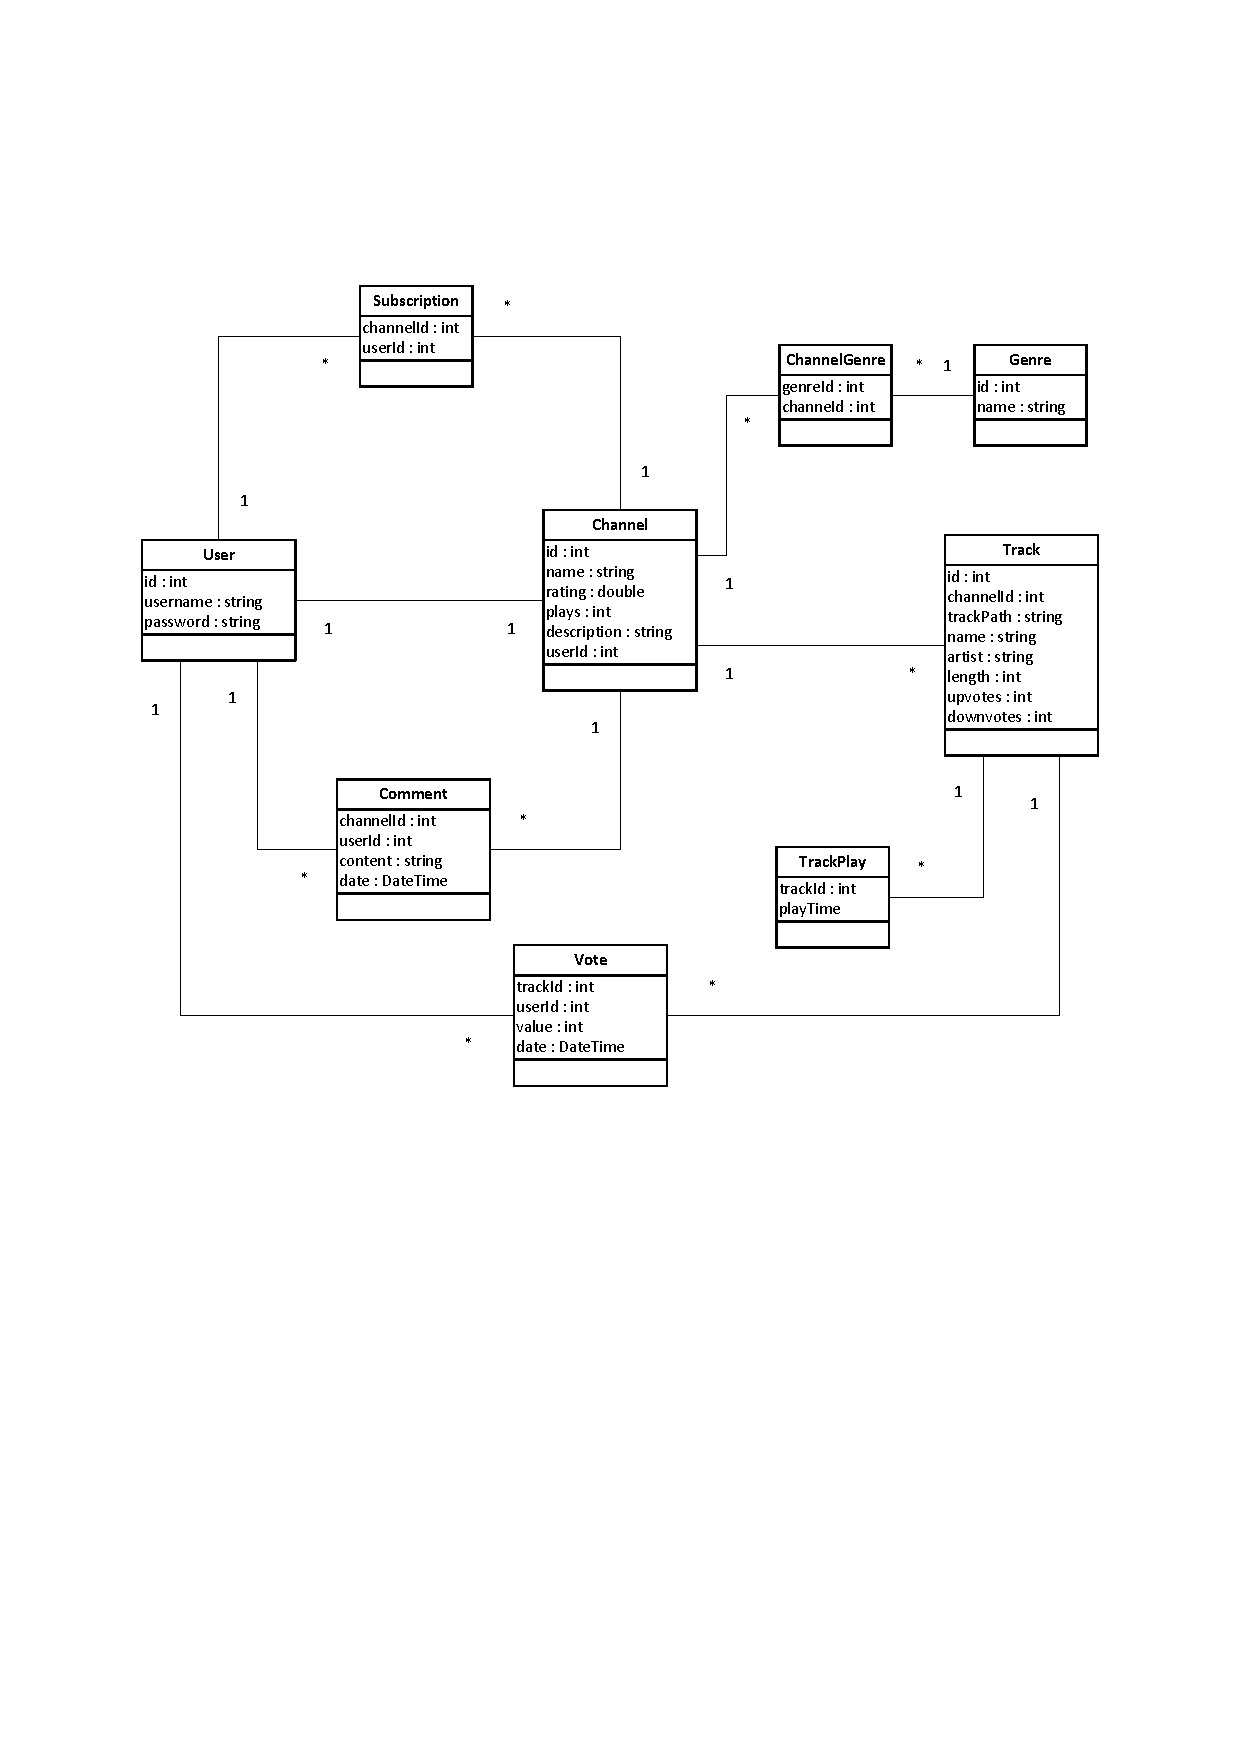
\includegraphics[width=420pt,keepaspectratio=true,trim=60pt 300pt 60pt 80pt]{./ermodel.pdf}
\caption{Data model of data entities}
\end{figure}
\subsection{Data storage}
For storing information about our data classes. Microsoft SQL Server has been chosen because it is integrated with the server. The reason for choosing a DMBS\footnote[1]{Abbreviation for Database Management System} to store most of our data in is because it is fast and optimized for storing and retrieving data. However a research paper\cite{Russel} suggests that when it comes to an object with a size beyond 1 MB it is faster to store the object on the file system. Due to the knowledge acquired from the paper we chose to store our music files on the file system, because the average size of an MP3 file is around 3-4 MB. A reference to the file system is placed in the database entities to connect files to table rows.

\subsection{Webservice}
In this section, we will analyse the WCF webservice. We will start be analyzing the architecture of the webservice and then we will analyse the design of the webservice methods.  \\*

\textbf{Webservice methods} \\*
The return types of most methods are intuitive. Methods which have at most one result will return the corresponding object, or a wrapper object in case it is an object which should reflect an object in the database, such as a channel or a user. \\
With methods which typically have more than one result, we have more options (methods like GetTrackIds and GetChannelIds). 
The first option is to return an array of the ids of the result. The second option is to return an array with all the objects associated with those ids. And the third option would be to return lazy objects, which were first completed (retrieved from the server) when the client called the object's methods. By returning an array of ids we allow the client to decide which objects they actually want to use time and bandwidth on retrieving completely. By returning all objects we force the instantiation of all objects in the server. And by using lazy objects we allow low bandwidth and only a single network transfer at first and wait until the objects are actually needed.
The returning of ids give the clear advantage of giving complete control to the client. When the client retrieves an array of ids, it can decide for itself which objects it actually needs. The disadvantage for this is that our webservice API needs methods for retrieving single objects from id and the client have to call this method for each object it needs. \\
The advantage for sending all objects back in the first method call is that there will only be one method call and only one network-transfer. The disadvantages is that this could get really rough on the bandwidth and server load as some objects might contain images and other types of heavy properties and all objects would have to be completely instantiated. Another thing is that the client would have to handle this, possibly, huge load of objects even though it might not need to use most of them. \\
The advantage of lazy object instantiation is that it potentially loads fewer objects. The actual object instantiation and retrieval is done when it is needed the first time. A massive problem with this is, that the load times would be unstable even when the site is completely loaded. Simple clicks or hovers, which requires some new information, would have to make a new network transfer. \\
We have chosen to implement the solution which returns ids. This allows for several network transfers but the possibility of making the workload on the bandwidth and the server as low as possible for what is actually required. The problem with lazy objects is that we assume that users want a fully loaded website to actually be completely loaded and not have to wait for some objects, which is shown to be there, but isn't actually loaded. \\
In the method GetChannelIds (the method used for searching in all channels) we have chosen the input to be an instance of SearchArgs. The SearchArgs class contains properties for all the different arguments we allow to search on, this way we have one method which takes one argument, rather than a method which takes parameters for every single property we have in SearchArgs. \\
All objects we return, which is a representation of data from our database, will be returned as a customized wrapper object. This is in order for us to be in complete control of what we return to our clients and in order to keep our internal structure as hidden as possible. If we returned raw objects created by our entity framework, we would expose data which is not relevant for the user and which could be used for malicious purposes, for example filesystem paths.

\subsection{GUI Technology}
A major part of our web-client is the GUI(Graphical User Interface) and the choice of GUI technology and framework will have a great influence on our project. In the analysis phase, before we start the initial design of the GUI, we choose several different criteria for a great GUI framework:
\begin{itemize}
\item Familiarity - How familiar the programming team are with the technology or a related technology?
\item Features - Does the technology have the features needed to support the features of our application?
\item Support - Is the technology widely supported on different browsers and in different web environments?
\item Extensibility/maintainability - Is the technology easy to maintain and extend and does it live up to common principles for good coding style, such as GRASP(General Responsibility Assignment Software Patterns)?
\end{itemize}
With these criteria defined, we consider several different GUI options:

\subsubsection{Silverlight}
Silverlight is a framework for creating rich web-applications and is especially known for its great streaming abilities(used by Netflix among others). A Silverlight application is declared in the Extensible Application Markup Language(XAML), the same language used for writing WPF applications.  Silverlight is fully integrated with Visual Studio and C\#, which is the language and IDE we are using to develop our web-service and the rest of our program. The developers in our team are very familiar with C\# and the .NET framework and has previous experience with Silverlight as well. The great streaming capabilities of Silverlight could also come in handy in our online radio-station application. Silverlight is not nearly as widely supported as other frameworks, such as ASP.NET or HTML5. It is often a necessity to download the Silverlight plug-in before you can use it. Recently, it has also been announced that Microsoft will stop to support Silverlight on future products, in favor of newer technologies.

\subsubsection{HTML5}

HTML is the common markup language used on the internet. Before HTML5, HTML was a reasonably promotive markup-language, that neede other languages and frameworks, such as JavaScript or Flash to implement more advanced features like video-streaming. With the introduction of HTML5, the language more advanced and now supports both video and audio-streaming, as well as SVG-graphics. HTML is the most widely used standard on the internet and even though HTML5 is not fully supported on every web platform yet, there can be no doubt that it will be soon. Because of its wide distribution, almost every other technology plugs well into it and there is a large amount of support to be found on the internet. The development team had no previous experience with HTML5 and would have to go through a learning process to be able to use it. Though HTML5 is much more advanced than the previous versions of HTML, it would still require another language, such as JavaScript, to use more advanced features, as well as a server side language for the “code-behind” operations.

\subsubsection{ASP.NET}
Asp.Net is a server-side framework developed by Microsoft and is used to dynamical create web-sites. It is a complete solution to creating a website with a build-in code-behind file written in C\#. ASP.Net is very well integrated with Visual Studio, which is the IDE, that the development team is mostly familiar with. It creates a complete solution to the website, without need for supporting languages, such as JavaScript or PHP. It is widely supported on most browsers. Compared to Silverlight, it does not have the same streaming capabilities. The styling of components are not that pretty and might require some extra work.

\subsubsection{Microsoft MVC}

Microsoft MVC\footnote{Abbreviation for Model View Controller} is a framework used to make ASP.NET websites structured in a model-view-controller pattern. It enables you to create very dynamic websites in a way that lives up to many of the GRASP\footnote{Abbreviation for General Responsibility Assignment Pattern.} principles for good and clean coding. With MVC you can create websites, that are easy to extend and maintain. Because the different components of the website are decoupled from one another, you can test these individually and utilize a lot of the unit testing tools available. It is a more advanced way to create a website, that requires some knowledge and experience to use.
Our choice
\\ \\
We choose to use the MVC framework. Even though that it requires a learning period for the development team to master it, we find that the benefits that the framework gives outweigh it.  It gives us the most possibilities for making a dynamic and well structured website. Some of the other GUI technologies are more simple, lightweight and easy to use, but they lack a lot of the structure and dynamic, that MVC has. For styling of the website, we use the Bootstrap layout, developed by Twitter. Bootstrap is not a framework, but simply consist of JavaScript files and CSS files, that styles the HTML elements. It is a simple and slick layout, that already has a lot of the styling we need.

\subsection{Track selection}
The functionality of choosing tracks that users prefer to listen to are crucial to the success of the system, as defined in the requirements R1 and R2. To make a preferable choice of which track to play next, the parameters that are considered when choosing are defined. The data model allows storage of when tracks has been played, up votes and down votes and tracks. From these entities, the following constraints are defined:
\begin{itemize}
\item The last X tracks played cannot be played again, as users want to listen to a variety of tracks in a short time perspective.
\item A track cannot be played more times than Y percentage of the total number of plays of a channel, to force variety in a long time perspective.
\item The frequency that a track is played at shall be affected by the up votes and down votes. A down vote and an up vote shall have an equal but opposite effect.
\item The selection of a track shall involve randomness to make the system less predictable.
\end{itemize}
The persistence of plays on a channel can be limited to Z days to limit the amount of data in the database. This does not limit the ability to choose a preferable track. The track selection shall happen as late as possible to make votes have an immediate effect on the track selection. 

\section{Implementation}
This section describes how the system is implemented by describing class responsibilities and collaborators, as well as the functional dynamics of the system. Complicated functionality and use of third party software will be explained.

\subsection{Major components}
Here is a list of the major components of the server:

\textbf{DatabaseDao} \\*
Communication with the database is done through a single data access object. This object functions as a bridge between the database and the server program, and it enables basic CRUD\footnote{Abbreviation for Create, Read, Update \& Delete} operations on the database for the server program. This class deals with objects generated by the entity framework. \\*

\textbf{FileSystemDao} \\*
Communication with the filesystem on the server is done through a single data access object. This object functions as a bridge between the filesystem and the program on the server. It enables the same basic operations on the filesystem as the DatabaseDao does on the database, however it has fewer responsibilities, because most of our data is stored in the database. This class is often used in the same context as the FilePath class because all file paths are stored as fields of FilePath instances. \\*

\textbf{RentItService} \\*
All communication between clients and the server, except the streaming of audio, go through this webservice class. It supports all the operations necessary to fulfill the requirements for the program. All calls to this class are either propagated to the Controller or the StreamHandler \\*

\textbf{TrackPrioritizer} \\*
This class selects tracks to be played based on the constraints defined in the track selection analysis. The track prioritizer are described in ~\nameref{sec:tp}. \\*

\textbf{Controller} \\*
This class is the main point of entry for almost all program functionality. All calls directly related to CRUD operations goes through this class. It also converts objects from entity framework objects to DatabaseWrapperObjects.\\*

\textbf{StreamHandler} \\*
Manages all EzStream processes and operations required for starting, stopping and maintaining channels. Acts as a secondary controller for all streaming and calls the FileSystem- and DatabaseDao directly. \\*

\textbf{DatabaseWrapperObjects} \\*
These classes are used to limit the data that are transferred with the webservice. Objects generated by the entity framework has lots of references that our database does not contain directly and we want to avoid giving the client references as collections, but as ids. It also hides some of the data like track file path and user password.

\newpage
\subsubsection{Class diagram}
\begin{figure}[H]
  \centering
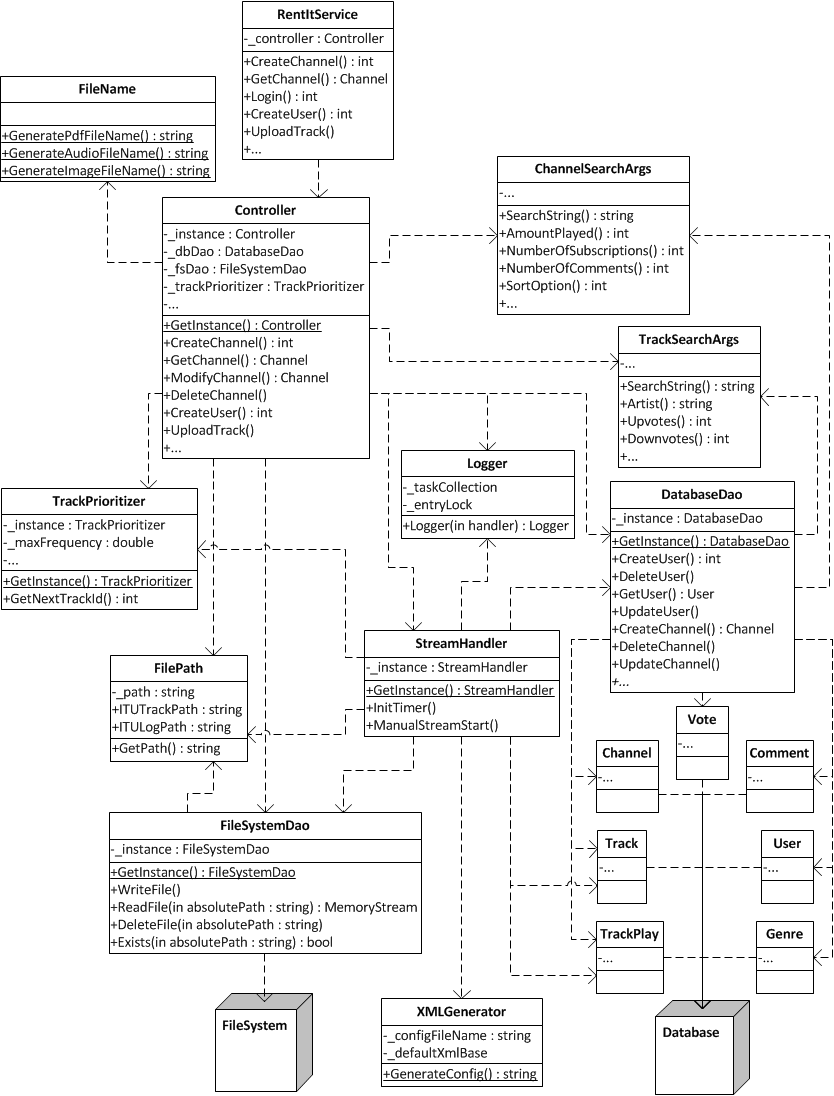
\includegraphics[width=450pt,keepaspectratio=true]{./ClassDiagramv2.png}
\caption{Class diagram of important methods and all classes}
\end{figure}

\subsubsection{TrackPrioritizer} \label{sec:tp}
The responsibilities of the track prioritizer was chosen with the idea that every time a channel should stream a new track, it should be selected as late as possible as described in the analysis. Hence the method that defines the main functionality(\texttt{GetNextTrack(...)}) of the track prioritizer returns only one track. However we encountered technical difficulties late in the process, making it necessary to extend the functionality of the track prioritizer to select entire playlists. The \texttt{GetNextPlayList(...)} method is therefore the method that the StreamHandler(the interfacing class) uses. The method calls \texttt{GetNextTrack(...)} a number of times until the accumulating playlist has a certain length. \\*

\textbf{Constants and variables} \\*
These constants and variables are used by the algorithm to determine the selection behaviour. Some of them are determined from the number of tracks and others always have the same value.
\begin{itemize}
\item \texttt{maxFrequency} defining the maximal percentage of times played a track can have to be selected for the next track. Based on the number of tracks.
\item \texttt{maxFrequencyLowerCap} defining the lowest possible value for maxFrequency.
\item \texttt{minimumRepeatDistance} the minimum amounts of tracks that shall be played before the same track can be played again.
\item \texttt{ratioConstant} defining the impact that votes has on the chance of a track being selected.
\end{itemize}
\textbf{The algorithm} \\*
The implementation of \texttt{GetNextTrack(List<Track> tracks, List<TrackPlay> plays)} is explained in the following section. \\*
At first the number of times that each track has been played is counted, and the percentage of number of times played is calculated. Any track exceeding more than the maximal percentage(\texttt{maxFrequency}) are not able to be selected as the next track. \\*
The number of tracks that can be selected are counted, and if there are less than or equal to the \texttt{minimumRepeatDistance} left to choose from, the minimum repeat distance are lowered. The \texttt{minimumRepeatDistance} latest tracks played are not able to be selected as the next track.  \\*
The eligible track's ratio are calculated from the formula:
\begin{align*}
ratio &= \frac{ratioConstant + upvotes}{ratioConstant + downvotes}
\end{align*}
The selection are visualized and explained in the following figure.\\
\begin{figure}[htp]
\centering
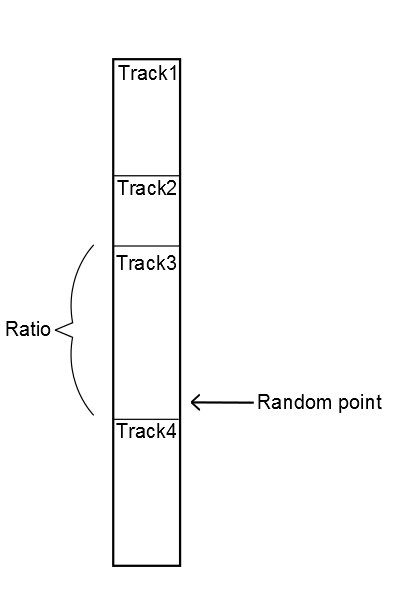
\includegraphics[width=130pt,height=200pt,keepaspectratio=true]{./trackSelectionB.png}
\caption{The pointer selects a random position along the height of the bar, and the track that the point belongs to is selected. The length that the track has are proportional to the ratio.}
\end{figure}
\textbf{ } \\*
\textbf{Time complexity} \\*
As the algorithm runs often, and in case of a \texttt{GetNextPlayList(...)} call, runs several times, the time complex is relevant. The algorithm iterates through tracks up to four times and track plays two times. The iterations does not involve iterations in iterations, making non of the \texttt{foreach()} calls quadratic in time. Therefore the time complexity is: 
\begin{align*}
\theta (g(n + m))
\end{align*}
Where \begin{math}n\end{math}, is tracks and \begin{math}m\end{math} is trackplays. As the time complexity is linear in the number of track plays there is no need for frequent removal of track play entities from the database.

\subsection{Third-party streaming components}
Two third party components have been used to to stream audio.
\subsubsection{IceCast}
To stream music we use a third-party server component named IceCast\cite{IceCast}, that streams multiple audio streams to multiple listeners. IceCast publishes multiple streams by creating an URL for each stream. IceCast needs a source client to read audio files and transform them to audio streams that can be played. Source clients connect to IceCast and it transmits the streams over the network. A running IceCast program is a requirement for our system to function.
\subsubsection{EzStream}
EzStream\cite{EzStream} is a source client used to transform audio files to audio streams. EzStream does not re-encode the audio stream, making it consume very few CPU resources. As we want to run as many channels as possible, and one channel requires one EzStream process, this is very important for keeping the server processor requirements low. To stream audio, EzStream takes a command line input referring to an XML document, specifying where the MP3 file or m3u file is located and which properties it shall use to connect to IceCast. \\ \\
\textbf{Interfacing with the server} \\
Mikkel du skal skrive det her for det kan du lide
Skriv om EzProcess, hvordan vi manager inputs or outputs fra process og hvordan vi restarter channels på bestemte tidspunkter.

\section{Testing}
This section will explain how we went about testing our software; it will start with a description of our testing strategy and the reasons behind it being
as it is; following with a description of how we tested against the requirements of the product, followed by our assessment on whether the program meets it's requirements.

\subsection{Testing strategy}
The most common way to test software, is by running unit tests, integration tests and system tests. Often it start with unit testing, which is about testing individual code units; following unit testing is integration testing that combine several software modules which are tested as a group. The RentIt project is not large enough be be comprised of
several sub-modules, so integration testing would be equal to system testing which is basically to black box test the entire program which is already completed
through the testing of GUI functionality.
\\*
That left us with unit testing on the server-side software. Contrary to usual test-driven development, we postponed the testing of many code units to near
the end of the project. The rationale behind this decision was that there was no way of creating a viable prototype without having implemented most of the 
functionality; in fact it was true for a large number of methods that simply implementing them on the spot would be just as fast as making method stubs 
that contained the intended execution flow. One could even argue that it was better this way, as one was forced into re-evaluate the structure of the webservice
interface, often resulting in an expansion or modification of operation contracts. \\*An important reason why unit tests are very relevant late in the process is the non-functional Supportability requirement 
\textit{"The impact on existing functionality of extensions and modifications shall not take more than an hour to discover for an educated software developer."}.
This is achievable with unit tests because they take less than an hour to run and confirms that all server side functionality works as intended.
\\*
This postponing of testing have drawbacks though, resulting in not every code unit having an associated unit test. While developing methods which are dependent on other untested methods, eventual errors are harder to find. This can slow development. It was prioritized to unit test the
critical code units in the "Controller" class and the "TrackPrioritizer" class because there complexity makes them very likely to be erroneous.\\ \\*
\textbf{Format and purpose of unit tests}\\*
Unit tests follow the following signature template:
\\*
\verb|public void <Tested class>_<Tested method>_<Parameter Type>_<Parameter Value>|
\\*
\verb|public void <Tested class>_<Tested method>_<State>_<State Value>|
\\*
An example of a parameter type could be password for Login, and parameter value could be null. \\*
This parameter testing approach insures that all exceptions are thrown and all correct behaviour are implemented. In between each unit test, all data in the database are removed and it is filled with test data, to make the testing environment more realistic, and to decouple tests. If Login is to be tested, it has to create a user first. If a user is already there, we can keep the unit test as simple as possible, only testing for Login. Keeping the unit tests simple makes it easier to locate an error. \\ \\
\textbf{System testing}\\*
Every test not contained in the unit test project are done manually. All testing on the graphical user interface are done by reviewing every single use case and trying all possible outcomes. The unit tests insures that the server functionality works, making it easier to locate an error with manual GUI testing. This is further described in the testing of functional requirements.

\subsection{Testing of specific requirements}
In this section, the fulfilment of each functional requirement are assessed and any directly related non-functional requirement are considered. \\ \\*
\textbf{General notes on the requirements} \\*
The non-functional requirements, U1 and U2 has not been meet for any of the functional requirements. \\ \\
\textbf{R0} \\*
\textit{The system shall allow all users to create a channel, add attributes, edit and delete the channel.} \\*
On the server side this is ensured with the unit tests:
\begin{itemize}
\item Controller\_CreateChannel\_...
\item Controller\_UpdateChannel\_...
\item Controller\_DeleteChannel\_...
\item Controller\_IsChannelNameAvailable\_...
\end{itemize}
UpdateChannel does also contain functionality for adding genres to it. In combination with the manual testing of the GUI, we assess that all the functional aspects has been completed, except for adding genres(F1), which is not implemented. Therefore more functionality has to be added and more usability testing has to be done before this requirement is fulfilled.\\ \\
\textbf{R1} \\*
\textit{The system shall allow users to listen to an online radio-channel that streams audio.} \\*
This requirement are not automatically tested, because there is no verifiable output that unit tests can assert on. However the requirement have been manually tested in context of the I2 non-functional requirement, which we feel has been meet. The F2 and F5 requirements has been manually tested and has been meet. F5 was tested by gathering multiple computers connected to different networks and make them stream the same channel. For the current state of the system we feel that this is sufficient, however the lack of automated tests violates the S3 requirement, hence making the extension of functionality more expensive. \\ \\
\textbf{R2:} \\*
\textit{The user shall be able to rate a track associated with a channel by up voting and down voting.} \\*
On the server side this is ensured with the unit tests:
\begin{itemize}
\item Controller\_CreateVote\_...
\item Controller\_DeleteVote\_...
\end{itemize}
With the manual GUI tests, this requirement has been fulfilled. Simple empirical testing reveals that the directly related functional requirement F3, F4 and U4 has been meet. \\ \\
\textbf{R3:} \\*
\textit{It shall be possible for users with a channel to upload a track to it.} \\*
This requirement clearly lack automated tests. The manual testing confirms that it works and that Re4 and F7 has been fulfilled. It is hard to test Re2, because of the various ways a server could fail. However our best assessment is that the Re2 is fulfilled and the implementation of the requirement is sufficient for the current state of the system. \\ \\
\textbf{R4:} \\*
\textit{It shall be possible for users to subscribe and unsubscribe to channels.} \\*
On the server side this is ensured with the unit tests:
\begin{itemize}
\item Controller\_Unsubscribe\_...
\item Controller\_Subscribe\_...
\item Controller\_SubscribeGetSubscriptions\_...
\end{itemize}
The very thorough unit tests made for the requirement confirms that the server side has meet the requirement. The manual tests shows similar results for the GUI. F4 are tested with unsubscribe state unit tests. All aspects of this requirement has been meet. \\ \\
\textbf{R5:} \\*
\textit{It shall be possible for user to comment on channels.} \\
On the server side this is ensured with the unit tests:
\begin{itemize}
\item Controller\_CreateComment\_...
\item Controller\_DeleteComment\_...
\end{itemize}
The unit test confirms that the server side meets the requirement. Manual testing has been done and because of the limited amounts of outcome, we are very sure that this requirement has been completely fulfilled. \\ \\
\textbf{R6:} \\*
\textit{It shall be possible to create, delete and edit accounts. All attributes of an account shall be editable.} \\*
On the server side this is ensured with the unit tests:
\begin{itemize}
\item Controller\_Login\_...
\item Controller\_SignUp\_...
\item Controller\_DeleteUser\_...
\item Controller\_IsCorrectPassword\_...
\item Controller\_IsUsernameAvailable\_...
\item Controller\_IsEmailAvailable\_...
\end{itemize}
According to automated and manual test this requirement has been meet. However it is questionable whether F10 has been meet. All intended usage requires authentication, but because our system is so insecure, it is easy to use it without authentication. \\ \\
\textbf{R7:} \\*
\textit{It shall be possible to search channels by a number of parameters, including number of subscribers, number of listeners, genres and name.} \\*
On the server side this is ensured with the unit tests:
\begin{itemize}
\item Controller\_GetChannelsWithFilter\_...
\end{itemize}
According to automated and manual test this requirement has been meet, except for searching for genres.

\subsection{Testing conclusion}
The testing conclusion clarifies and concludes in which degree the functional and non-functional requirements have been meet and in which degree it is possible to assess it. \\*
The genre aspect of the functional requirements are implemented server side, but not client side, making every functional requirement related to it incomplete. Every other fundamental functionality has been implemented and tested. \\*The automated testing of some of the functional requirements lacks, making the S3 non-functional requirement unfulfilled, and the general certainty of whether the system is flawless unsatisfying.\\*The logging requirements F8 and F9 are mostly meet. Not every exceptional state and state change are logged, but most are. U1 and U2 are totally unfulfilled, while U3 and U4 are completely fulfilled. The reliability requirements requires a lot of effort to test, which we have not done. However we have not experienced any violation of it. Therefore we assess that they are meet, but also that we cannot be sure of it. The implementation non-functional requirements are meet.

\section{Collaboration with SMU}

\subsection{Interaction with the ITU system}
As both the ITU system and the SMU system is an IS\footnote[2]{Abbreviation for Information System} and deployed on the same server, some of the classes have been reused in the SMU system and the ORM\footnote[3]{Abbreviation for Object Relation Mapping} is in the same entity framework.
The classes that have been reused are in the utilities namespace, and are FilePath, FileSystemDao and Logger. We have designed the classes in such a way, that a method call in one system can't affect the other system. \\
A success criteria for our systems is that an error or change in one system should not affect the other if not intended. Two different web services have been used to avoid that an erroneous method affects the other system.
The drawback to this decision is that the clients cannot share web service methods without adding the other web service. However, none of the clients need the web service of the other system. 

\subsection{SMU webservice api}
The group from Singapore Management University requested the following API.

\begin{itemize}
	\item \texttt{int SignUp(string email, string name, string password, bool isAdmin)}
	\item \texttt{int LogIn(string email, string password)}
	\item \texttt{User GetUserInfo(int userId)}
	\item \texttt{User UpdateUserInfo(int userId, string email, string username, string password, bool? isAdmin)}
	\item \texttt{void DeleteAccount(int userId)}
	\item \texttt{Book[] GetAllBooks()}
	\item \texttt{Book[] GetPopularBooks()}
	\item \texttt{Book[] GetNewBooks()}
	\item \texttt{Book[] SearchBooks(String searchString)}
	\item \texttt{Book[] GetBooksByGenre(String genre)}
	\item \texttt{Book GetBookInfo(int bookId)}
	\item \texttt{int HasRental(int userId, int bookId)}
	\item \texttt{Rental[] GetRental(int userId, int bookId)}
	\item \texttt{int RentBook(int userId, int bookId, int mediaType)}
	\item \texttt{MemoryStream DownloadPdf(int bookId)}
	\item \texttt{MemoryStream DownloadAudio(int bookId)}
	\item \texttt{MemoryStream DownloadImage(int bookId)}
	\item \texttt{Rental[] GetActiveUserRentals(int userId)}
	\item \texttt{Rental[] GetAllUserRentals(int userId)}
	\item \texttt{void DeleteBook(int bookId)}
	\item \texttt{int UploadBook(string title, string author, string description, string genre, double price, MemoryStream image)}
	\item \texttt{Book UpdateBook(int bookId, string title, string author, string description, string genre, double? price, MemoryStream image)}
	\item \texttt{void UploadAudio(int bookId, MemoryStream mpMP3, string narrator)}
	\item \texttt{void UploadPdf(int bookId, MemoryStream pdf)}
\end{itemize}

\subsection{Collaboration Considerations}
One of the main focuses of the RentIt project was our collaboration with another development team at Singapore university(SMU)[reference]. There are many risk factors and challenges associated with international collaboration, especially when the collaborators do not come from the same cultural background. Simple communication tasks, that we take for granted when communication within our own team, can easily become an issue when collaboration with a foreign team and the differences in work routines, traditions and culture often leads to frustrations and project setbacks. \\

In this section, we will not cover any of the technical details about the program we developed with the SMU. We will focus on how the communication went and how well we worked together as part of an international collaboration. We will use a lot of the theory from the book "Subgroups dynamics in internationally distributed teams" by Crampton and Hinds. We will first analyse the potential faultlines\cite{smu} between our development team and the team at SMU. Then we will discuss what we can do as team to avoid that these faulines evolves into problems. Last, we will conclude on how successful our collaboration with the SMU team were and suggest changes we would make in an potential future collaboration.\\

\paragraph{Data on SMU team}

This is the data initial data we get from the SMU wiki. The SMU team consists of 3 members.\\

\begin{itemize}
\item Waritta: Girl from Thailand
\item Umair: Boy from Pakistan
\item Safouan: Boy from Qatar
\end{itemize}

\subsubsection{Fault lines}
A faultline is defined as a difference between two subgroups, that can potentially lead to a conflict. A faultline does not necessarily have to lead to a problem, but like the continental lines of the earth they can suddenly erupt and become one. A faultline enhances the notion of “us and them”, also known as ethnocentrism\cite{smu}. We have analysed and identified the potential faultlines we see between the SMU team and us:

\paragraph{Geographical location}
The most obvious fault line is the difference in geographical location. The fact that all live in the same city and meet face to face on a regular basis is hugely different from our relationship with the SMUs, who we only see on a computer screen and communicate with through email and video chat. The difference in geographical is the fault line we measure all other fault lines against.

\paragraph{Gender diversity}
Our team is made up of only men, while the SMUs has one girl in their team. This makes their team a gender diverse team as opposed to ours.

\paragraph{Engineers/Designers}
The team at SMU university is responsible for the webclient, while we are responsible for the web-service. This division of work area creates a natural fault line between them and us. Us, as engineers who are handling data and logic, and them as designers working with windows and styling. The fact that our team has not had very much experience with web-design and the SMU teams smaller knowledge of web-services and backend programming, can lead to many misunderstanding and an ethnocentric view of our own subgroup. It can be tempting to blame the designers for not using the web service right, instead of putting an effort into understanding their website and modulating the web service to suit that as best as possible.

\paragraph{Social etiquette}
There is a large difference social norms in Denmark compared to those in Singapore. In Denmark we have a very casual tone in a work environment. We have a very homogenous society, where the difference between peoples social status is very small. We dislike hierarchies and talk to our superiors in the almost the same way, that we would talk to our colleges. In Singapore and many asiatic countries they have a much more strict social etiquette, where you behave a lot different when you are in an official environment compared to when you are in a casual, private environment. This difference can create a faultline between us and the SMUs. They might see us as rude and unprofessional, whereas we might see them as stiff and strict. 

\subsubsection{Solutions}
The fault lines we have identified in the previous chapter are all risk factors, that can create conflict between us and the SMU development team. It is important to address and prepare so that the risk of conflict is minimized as much as possible.

The situation we want to avoid is a situation of ethnocentrism. Ethnocentrism is when a subgroup sees itself as superior to the other group as acts in a hostile and competitive way against it. The more faultlines we have that aligns with the geographical separation of the two groups, the more strong the ethnocentric situation will be. The situation we want is a situation of ethnorelativism\cite{smu}. Ethnorelativism is a situation where a subgroup takes the perspective of the other group and tries to understand their situation. Each subgroup adapts to the context other subgroup and the notion that both development teams are part of one “overarching subgroup” is enhanced. What steps can we take to achieve this?\\

A good way to increase the ethno relativistic situation is to find the lines where our development team and the SMUs have something in common. \\

\paragraph{Students}
Both our development team and the SMU team consists of students. This gives us a lot of things in common. We all have to deal with exams, with the educational system, with deadlines and work. The fact that we have to deal with these things draws a faultline between us and them and the rest of the world, and thereby increases our sense of belonging to the same subgroup. This subgroup is further strengthened by the fact, that our educations are very much alike. \\

\paragraph{Age}
Both our team and the SMU team between 20 and 30 years old. Even though that the age in itself does not mean we have anything in common, it makes it likely that our general life situations are alike. We are more likely to have an outgoing lifestyle, to not have kids and to be somewhat “unsettled” in our lives so far. We will likely have many of the same pop-culture references and be interested in many of the same subjects. 

\paragraph{Language}
Both us and the SMUs have the english language in common. In both Singapore and in Denmark a reasonably high level of english is taught and spoken by the students. This gives us a good common ground for expressing ourselves and potentially enhances the feeling that we belong to the same subgroup. \\

In our communication with the SMUs, we must remember these commonalities and share them with the SMUs. Information sharing\cite{smu} is a way to build a more moderate and accurate picture of another subgroup. Often, fault lines are build on prejudice and these can be removed by the sharing of information across the subgroups. We must share information about our background, our lives as students and ask them about theirs. Multural Positive Distinctiveness(MPD)\cite{smu} is also a point we must address. If we define in our subgroup what we are good at, it is easier for us to accept another subgroup and respect their field of expertise. In our communication with the SMUs we must also give them credit for their field of expertise. \\

\subsubsection{Conclusion of the SMU collaboration}

We have analysed the Fault Lines and identified the ways to avoid them. How did the collaboration actually go? \\

\paragraph{Description of the collaboration }
In our first video session with the SMUs, the communication was very formal. It was a timeboxed meeting and we both had a teacher present outside the meeting room. In the next meetings the tone became more relaxed and casual. It turned out that none of the members of the SMU team came from Singapore, but from Thailand, Qatar and Pakistan, and it most likely had a big impact on the collaboration. Waritta and Safouan were the ones that lead the discussion from their part and Umair was much more silent. We quickly established that we were going to make a WCF webservice and that their job was to give us the methods and data management they needed for their client to function. After a couple of days they sent us their API and we started working. At their suggestion, we utilized a chat application called WhatsApp\cite{whatsapp} which gave us direct communication with each individual member of the SMU team. In between meetings we used this to engage in information sharing, both related to the project, but also casual talk. In this way we could learn about the members in the SMU team on a more personal level and helped to understand things from their perspective. Some of the members has even kept contact since we finished the project. Waritta was the one we had the most contact with and she seemed to be the one with the most knowledge about backend programming. They continuously sent us list of errors and exceptions in the program, and we tried to fix them as soon as possible. As we neared their deadline we had fixed most of the problems and when the deadline came, they seemed satisfied and we wished them good luck on their further process. \\

\paragraph{Conclusion on fault lines and solutions}
In this section we will conclude which faultlines that caused problems and which that remained invisible. \\

The fault line in geographical location was present and there was no way for us to avoid that. We communicated with the SMUs through a video conference and it sat a significant restriction on our communication. We had to be very precise about how we communicated our requirements to them, and we had to carefully analyse their responses and requirements to be perfectly sure that we understood it right. Time difference became less of a problem, since the SMU team were available almost all the time. \\

The fault line in gender difference was not very present. A major factor in that was the fact that the only woman in the SMU group was the one who had the most technical capabilities. That destroyed the classic fault line that says: “Women are designers, men are engineers”.\\

The faultline between us as engineers and them as designers were present, but not as much as it could have been. After the first meeting, we were concerned about the technical possibilities of the SMUs and we unsure how much of the technical work they expected us to do. After they sent us the first version of the web-service API that they needed, it became clear that they were not oblivious to the technical aspects of a WCF webservice and we became more confident in their technical abilities. As mentioned before, we had almost no technical communication with any members of the SMUs except Waritta and it created kind of a line between her and us as engineers and the rest of the SMU team as designers. It did not create any significant problems, though. \\

The fault line in social etiquette became a much smaller problem than first expected. Because they were not from the same country, they did not see themselves as a part of the same cultural group and therefore the line between us and them became much less deep. Many of the social differences, that we had found to be a potential faultline, turned out not to be a problem. The communication with them was very relaxed and informal and in between talking about the project, we engaged in casual talk about the weather, student life and parties. Even though that they were in a very different part of the world, it seemed that both them and us more identified with being students and being young, that with being from Denmark, Qatar or Thailand etc.\\

\paragraph{Final conclusion}
Our collaboration with the SMUs was a success. We did not run into major issues, that would create significant ethnocentrism in our group and the potential faultlines cause any major problems. Even though that we were divided geographically, we succeeded in working well together. We did run into problems, but most were problems related to the project itself and was not rooted in the fact that we were doing an international collaboration. The reason why it went well can be found in the fact, that the both our team and the SMUs were well prepared and responded very quickly to the emails and updates that we sent them. It can also be found in the fact, that the members of both groups were much more alike culturally than we had expected. A big factor can also be found in the fact, that the division of work between us and the SMUs was very well defined from the start. If our areas of work had overlapped more and there had been more mutual dependence, it would most likely have caused much more problems and frustrations from both parts. 

\paragraph{Changes in a future collaboration}
What would we do different in a potential future collaboration? One of things that would have helped the collaboration would have been access to the SMU website. Not so much because we wanted to influence any of their design choices, but because it would have given us a better understanding of the problems they were facing. Understanding the problems of the other team can help for a much better collaboration. The SMU team did supply us with information about what services they needed, but access to the actual website they developed would have been even better. In a future collaboration we would also emphasize direct communication, like the one we had through WHatsApp, even more. We would make sure that at least one member of our development team would always be available for questions. He would not have to be able to give a correct answer all the time, but the fact that you get a very quick response as soon as possible really helps to increase the feeling of collaboration. It is important that the team feels as less secluded as possible and that the waiting period between questions and answer is limited as much as possible. 

\begin{thebibliography}{9}
\bibitem{Russel}
  Russell Sears, Catharine van Ingen, Jim Gray
  \emph{To BLOB or Not To BLOB: 
Large Object Storage in a Database or a Filesystem}.
  Microsoft Research and University of California at Berkeley
  April 2006
  
\bibitem{smu} Crampton and Hinds \emph{Subgroups Dynamics In
Internationally Distributed
Teams: Ethnocentrism Or
Cross-National Learning? } 2005
	
\bibitem{whatsapp} http://www.whatsapp.com \emph{www.WhatsApp.com}
	
\bibitem{IceCast}
  www.xiph.org, the xiph open source community
  \emph{www.IceCast.org, IceCast documentation and contact}.
    
\bibitem{EzStream}
  www.xiph.org, the xiph open source community
  \emph{www.icecast.com/ezstream.php}.
\end{thebibliography}
\newpage
\appendix
\section{Diagrams}

\begin{figure}[htp]
\centering
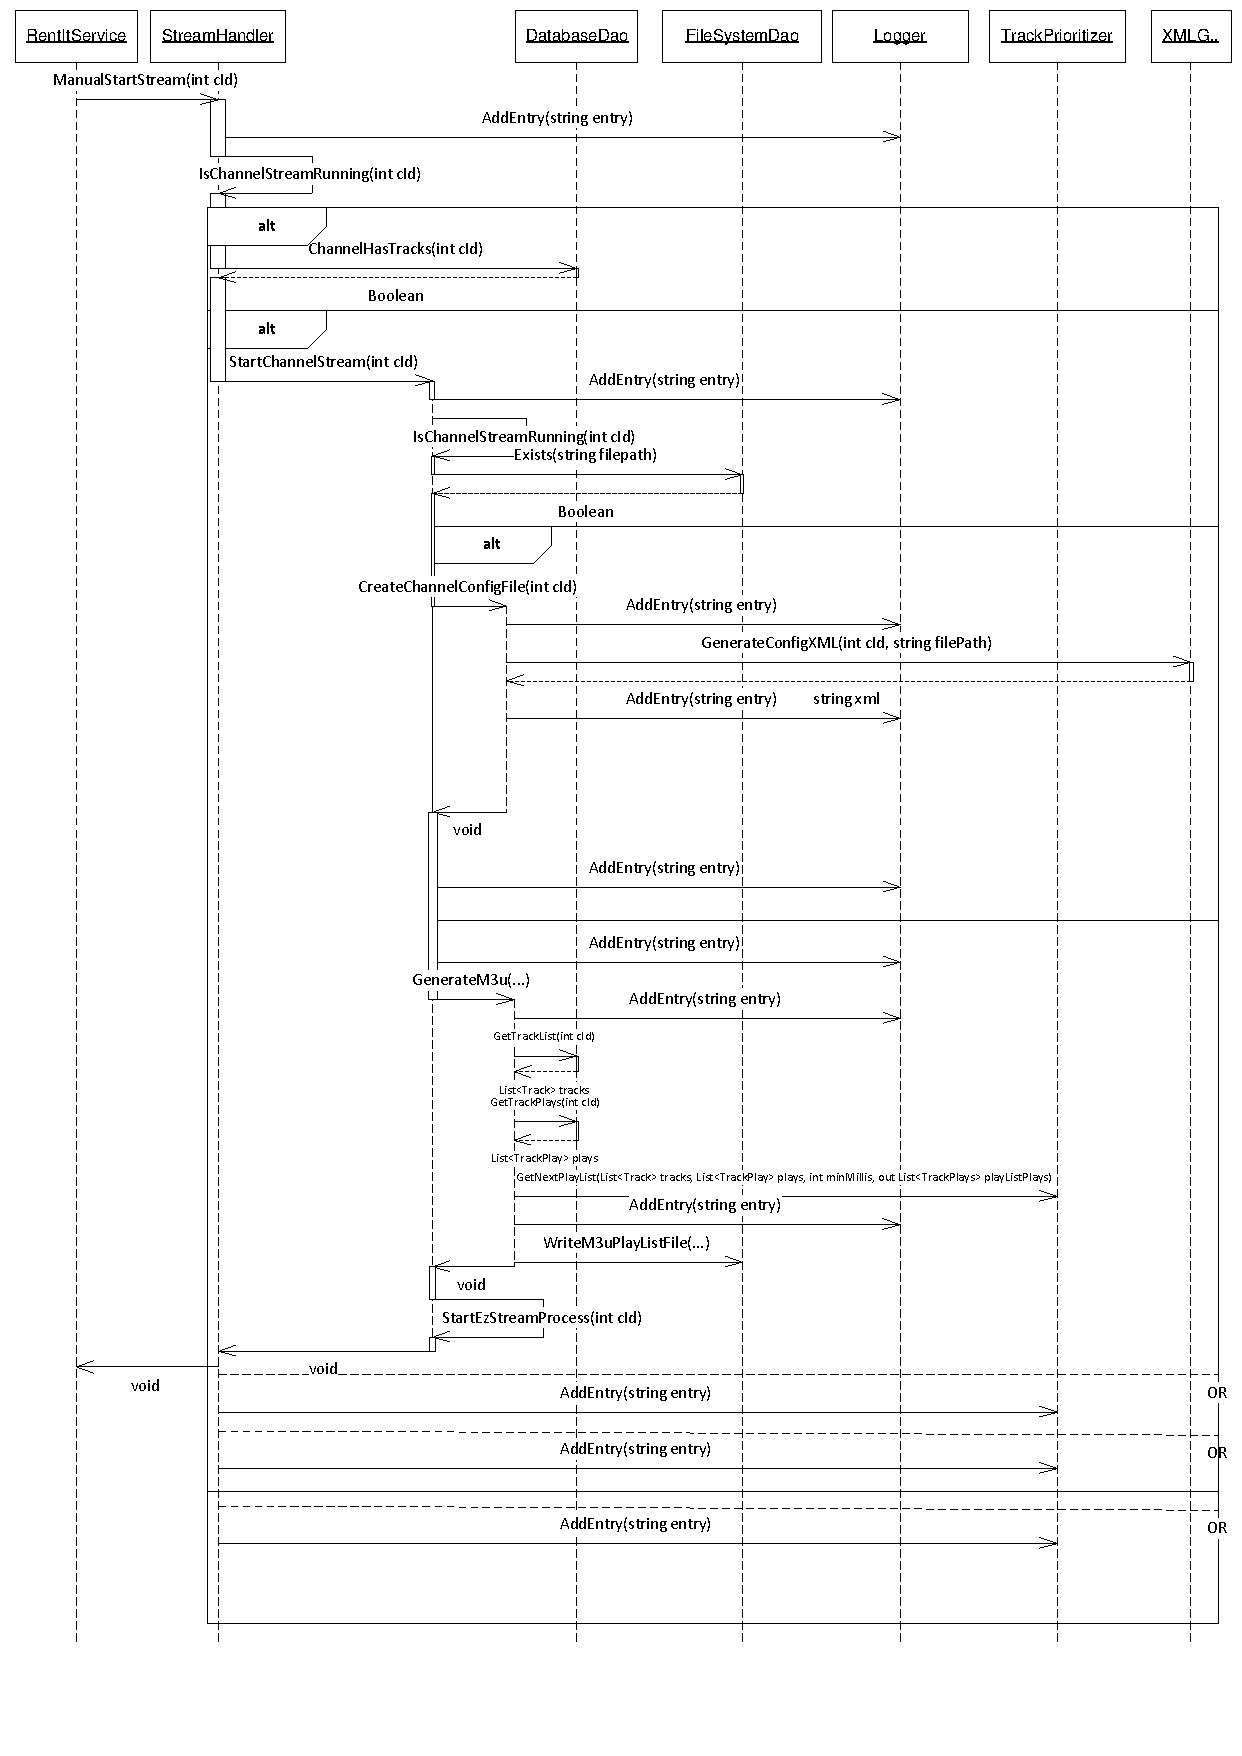
\includegraphics[width=17cm,keepaspectratio=true,trim=0pt 300pt 0pt 0pt]{./StartStreamSD.pdf}
\end{figure}

\begin{figure}[htp]
\centering
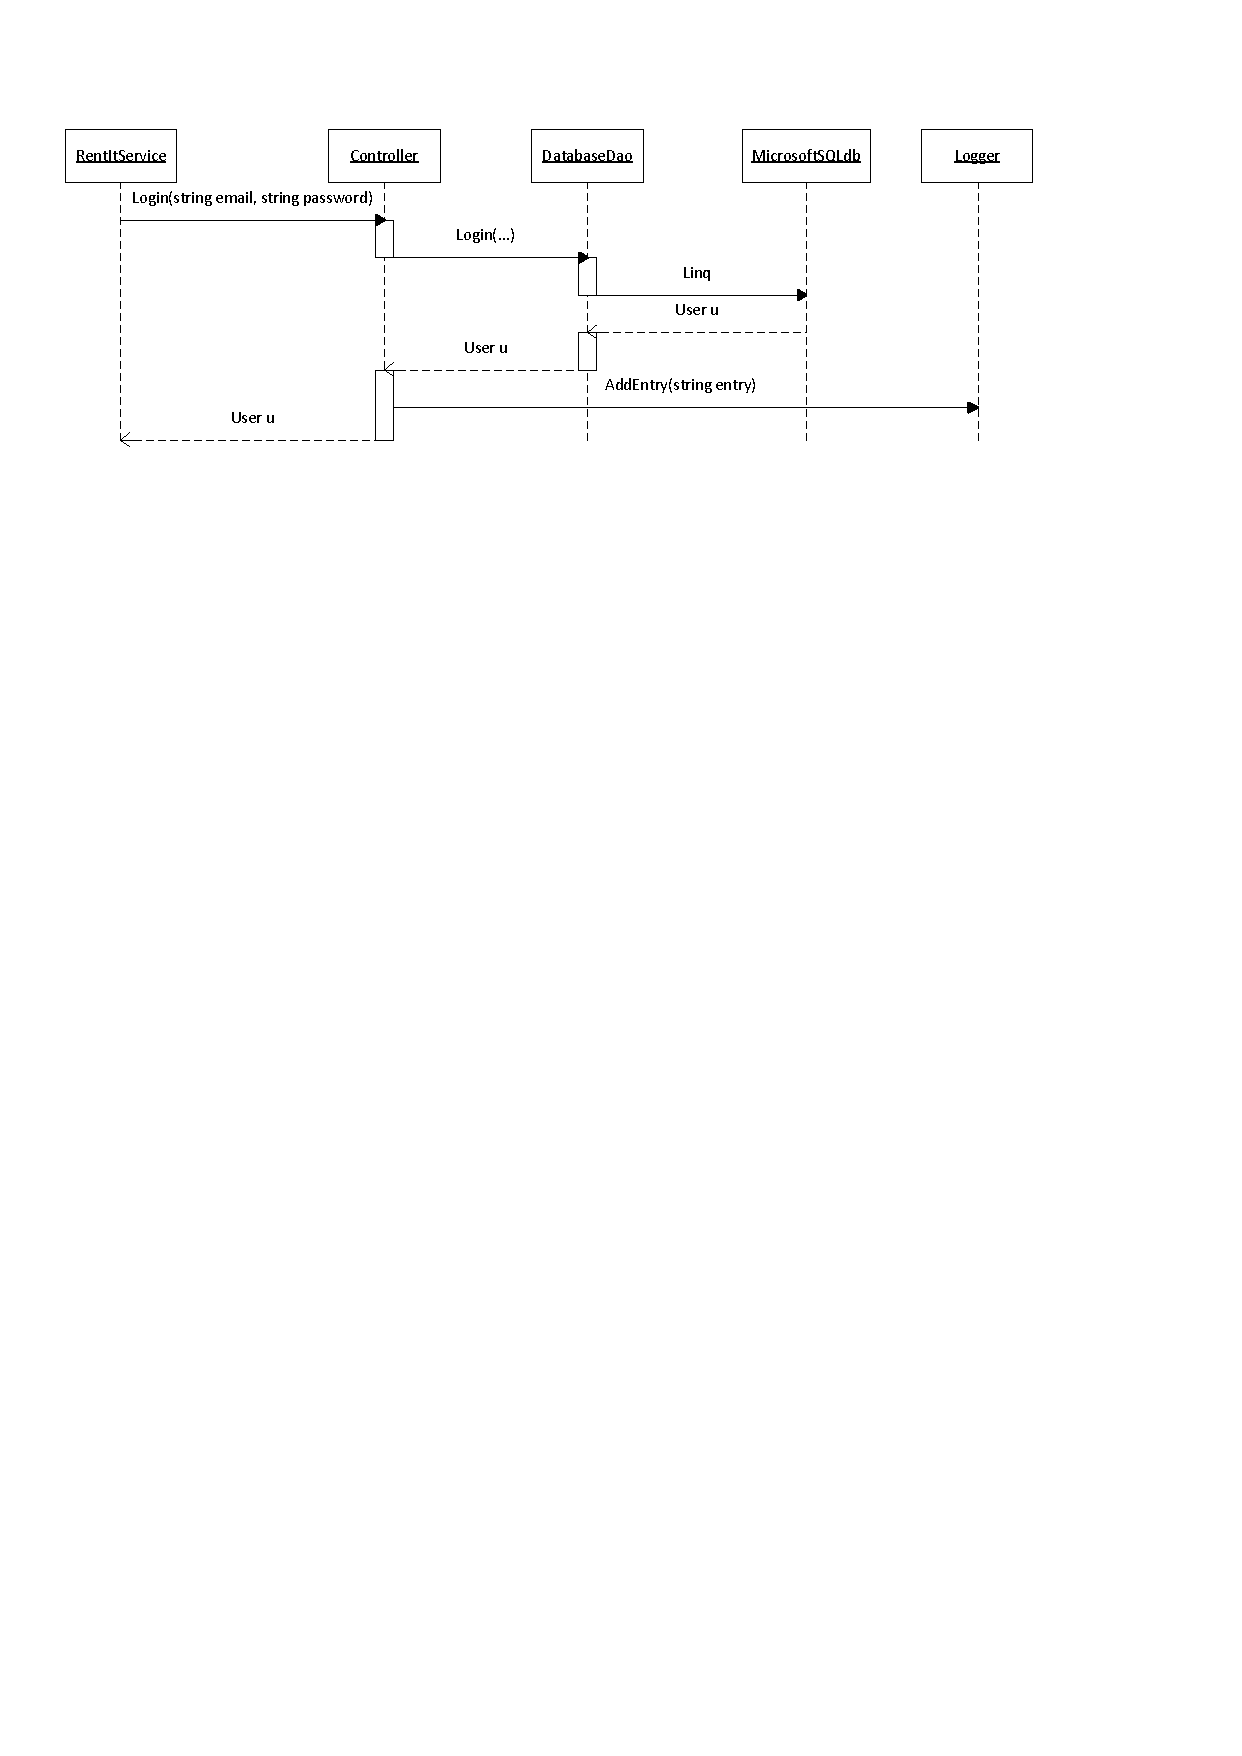
\includegraphics[width=17cm,keepaspectratio=true]{./LoginSD.pdf}
\end{figure}
\begin{figure}[htp]
\begin{tabular}{| l | l | l | l | l | l |}
  \hline
  Item & Mikkel & Mark & Toke & Morten & Andreas \\
  \hline
  \rowcolor{LightGray}\multicolumn{6}{|l|}{Documentation} \\
  \hline
  Introduction &  &\cellcolor{Gray} &\cellcolor{Gray}&  & \\
  \hline
  Use cases \cellcolor{Gray}& \cellcolor{Gray} & \cellcolor{Gray} & \cellcolor{Gray} & \cellcolor{Gray} & \cellcolor{Gray} \\
  \hline
  Functional requirements \cellcolor{Gray}& \cellcolor{Gray} & \cellcolor{Gray} & \cellcolor{Gray} & \cellcolor{Gray} & \cellcolor{Gray} \\
  \hline
  Non-functional requirements \cellcolor{Gray} & \cellcolor{Gray} &  &  &  &  \\
  \hline
  Target audience &  &  &  &  & \cellcolor{Gray} \\
  \hline
  Architecture &  & \cellcolor{Gray} &  &  &  \\
  \hline
  Data Model & \cellcolor{Gray} & \cellcolor{Gray} &  &  &  \\
  \hline
  Data Storage &  &  &  &  &  \\
  \hline
  WebService &  &  &  &  &  \\
  \hline
  GUI Technology &  &  &  &  &  \\
  \hline
  Track Selection &  &  &  &  &  \\
  \hline
  Major components &  &  &  &  &  \\
  \hline
  Class Diagram &  &  &  &  &  \\
  \hline
  Track Prioritizer &  &  &  &  &  \\
  \hline
  Streaming Components &  &  &  &  &  \\
  \hline
  Testing &  &  &  &  &  \\
  \hline
  Interaction with the ITU system &  &  &  &  &  \\
  \hline
  SMU webservice API &  &  &  &  &  \\
  \hline
  Collaboration considerations &  &  &  &  &  \\
  \hline
  Sequence Diagrams &  &  &  &  &  \\
  \hline
  Conclusion &  &  &  &  &  \\
  \hline
  \rowcolor{LightGray}\multicolumn{6}{|l|}{ITU-Server Code} \\
  \hline
  Server Controller &  &  &  &  &  \\
  \hline
  DatabaseDao &  &  &  &  &  \\
  \hline
  FileSystemDao &  &  &  &  &  \\
  \hline
  TrackPrioritizer &  &  &  &  &  \\
  \hline
  StreamHandler &  &  &  &  &  \\
  \hline
  Logger &  &  &  &  &  \\
  \hline
  DatabaseWrapperObjects &  &  &  &  &  \\
  \hline
  XMLGenerator &  &  &  &  &  \\
  \hline
  IRentItService/RentItService &  &  &  &  &  \\
  \hline
  SearchArgs &  &  &  &  &  \\
  \hline
  \rowcolor{LightGray}\multicolumn{6}{|l|}{Webclient Code} \\
  \hline
  Model &  &  &  &  &  \\
  \hline
  Views &  &  &  &  &  \\
  \hline
  Controller &  &  &  &  &  \\
  \hline
  Layouts &  &  &  &  &  \\
  \hline
  CSS &  &  &  &  &  \\
  \hline
  JavaScript &  &  &  &  &  \\
  \hline
  \rowcolor{LightGray}\multicolumn{6}{|l|}{SMU-System Code} \\
  \hline
  ISMURentItService/SMURentItService &  &  &  &  &  \\
  \hline
  SMUController &  &  &  &  &  \\
  \hline
  SMUDao &  &  &  &  &  \\
  \hline
  \rowcolor{LightGray}\multicolumn{6}{|l|}{Automated Test Code} \\
  \hline
  ItuController\_Test &  &  &  &  &  \\
  \hline
  ItuDao\_Test &  &  &  &  &  \\
  \hline
  TrackPrioritizer\_Test &  &  &  &  &  \\
  \hline
  FileSystemHandler\_Test &  &  &  &  &  \\
  \hline
  Logger\_Test &  &  &  &  &  \\
  \hline
  TestExtensions &  &  &  &  &  \\
  \hline
  SMUController\_Test &  &  &  &  &  \\
  \hline
  SMUService\_Test &  &  &  &  &  \\
  \hline
\end{tabular}
\end{figure}
\section{Glossary}
Track: An audio file that the users can listen to via channels. \\*
Channel: A collection of tracks that is played infinity, and can be listened to by users. Managed by a channel host.

\end{document}